\documentclass[12pt,a4paper]{article}
\usepackage{bold-extra}
\usepackage{appendix}
\usepackage{amsfonts,amsmath,amssymb}
\usepackage{enumerate}
\usepackage{float}
\usepackage{geometry}
\usepackage{graphicx}
\usepackage{latexsym}
\usepackage{listings}
\usepackage{multicol,multirow}
\usepackage{subfigure}
\usepackage{tabularx}
\usepackage{ulem}
\usepackage{tikz}
\usepackage{xcolor}
\geometry{a4paper,left=1in,right=1in,top=1in,bottom=1in}
\begin{document}
\centerline{\Huge{{\textbf{PHYSICS I\ \ Problem Set 2}}}}
\vspace{0.5cm}
\leftline{\large{Name: Haotian Fu}}
\rightline{\large{Student ID: 520021910012}}
\paragraph{\large \textbf{Problem 1}}~{\textbf{Solution}}
\vspace{2mm}\\
\noindent (a) Since the cable is not elastic, its length is constant. Therefore, based on the constant length, we have following relationships for pulley B
\begin{figure}[H]
    \centering
    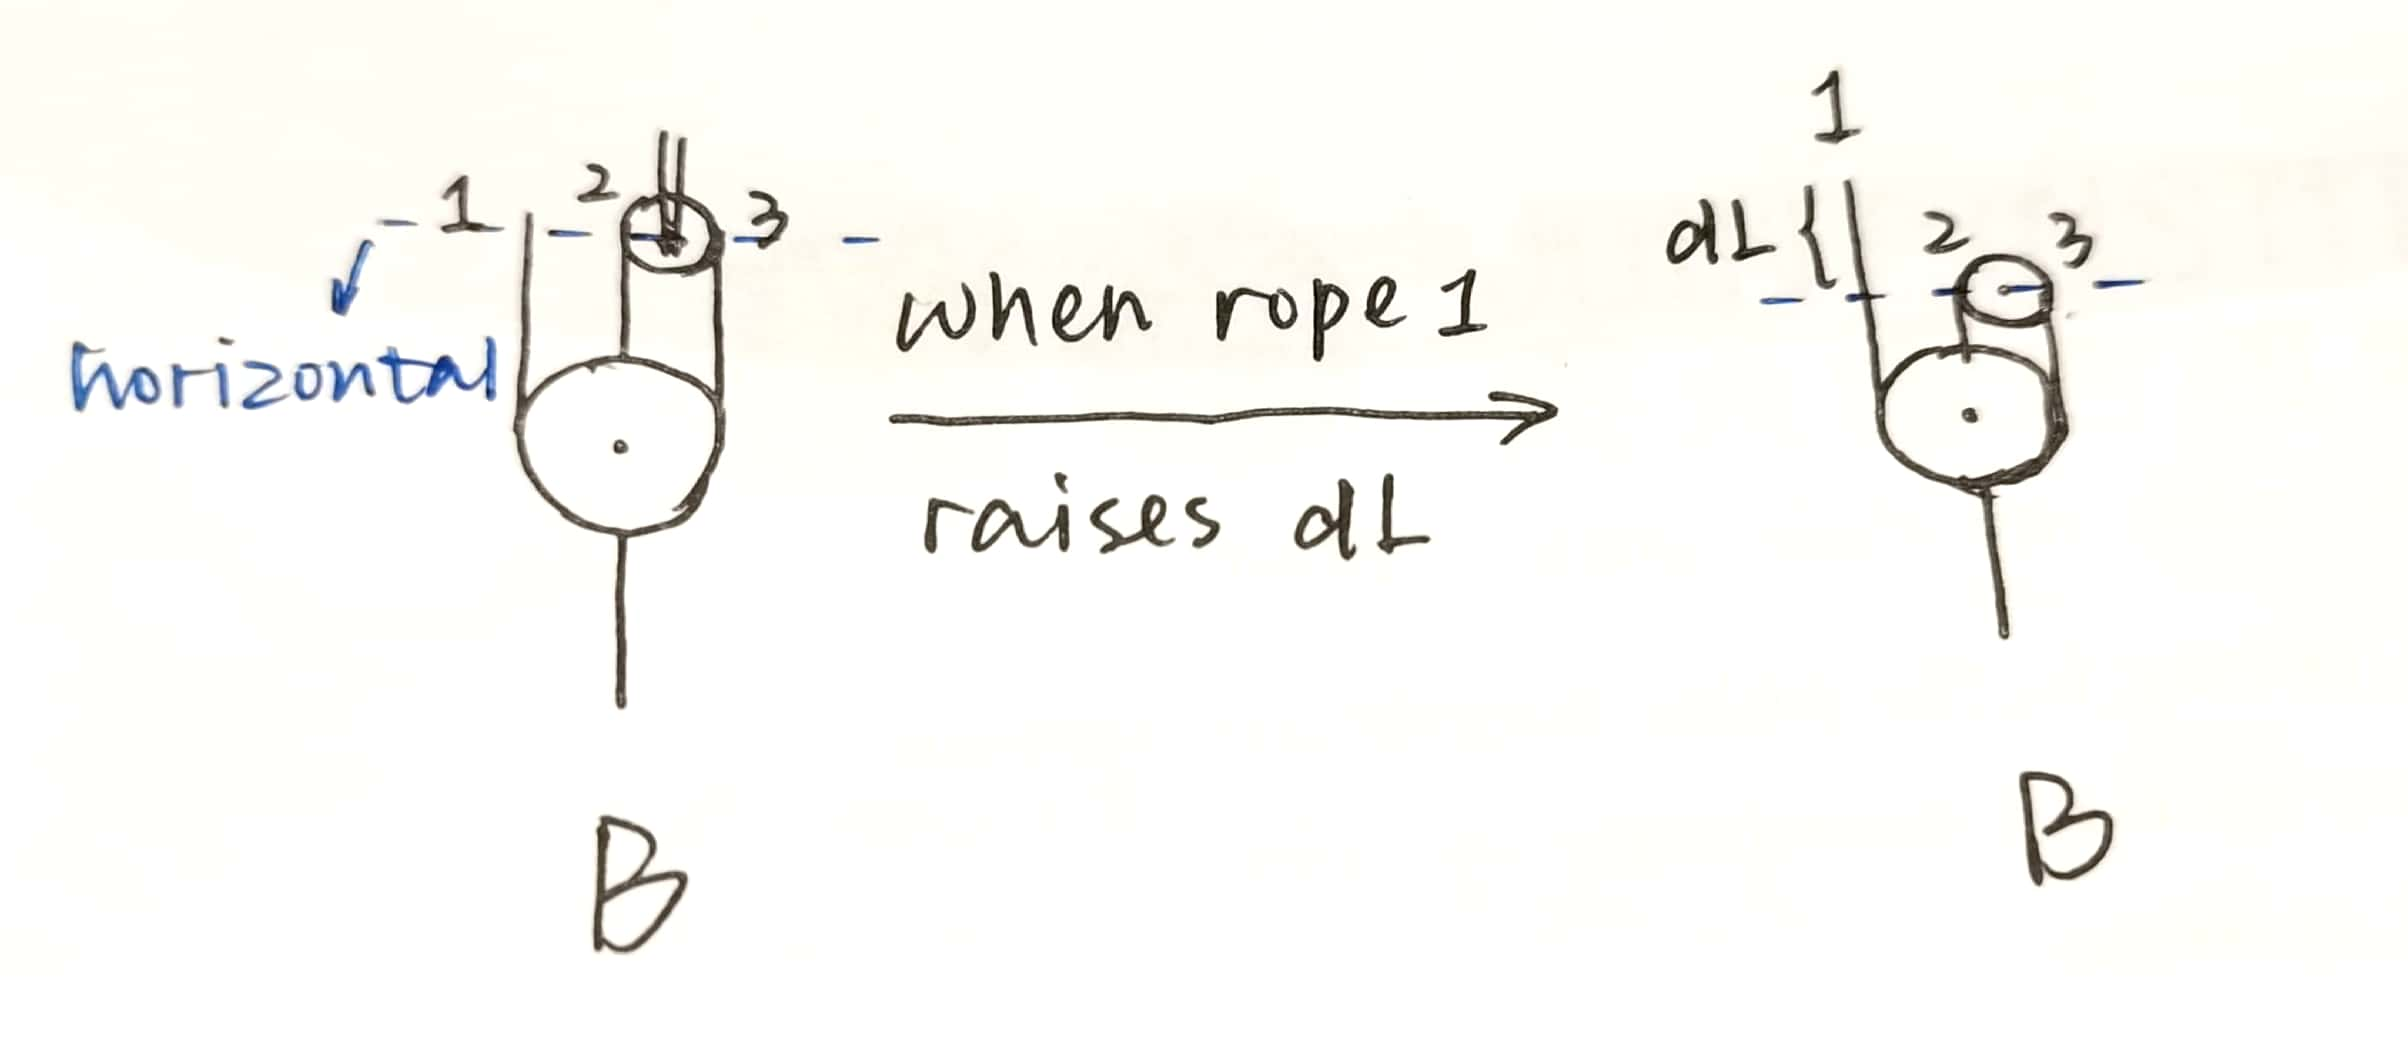
\includegraphics[height = 4cm]{1.jpg}
    \caption{Analysis of pulley B}
\end{figure}
\par According to Figure 1, it is evident that cables below the horizontal line (blue line in Figure 1) raise $\frac{dL}{3}$ on average when the rope 1 raises \textit{dL}.
\par Analogously, we take the pulley attached to \textit{L} as our observation.
\begin{figure}[H]
    \centering
    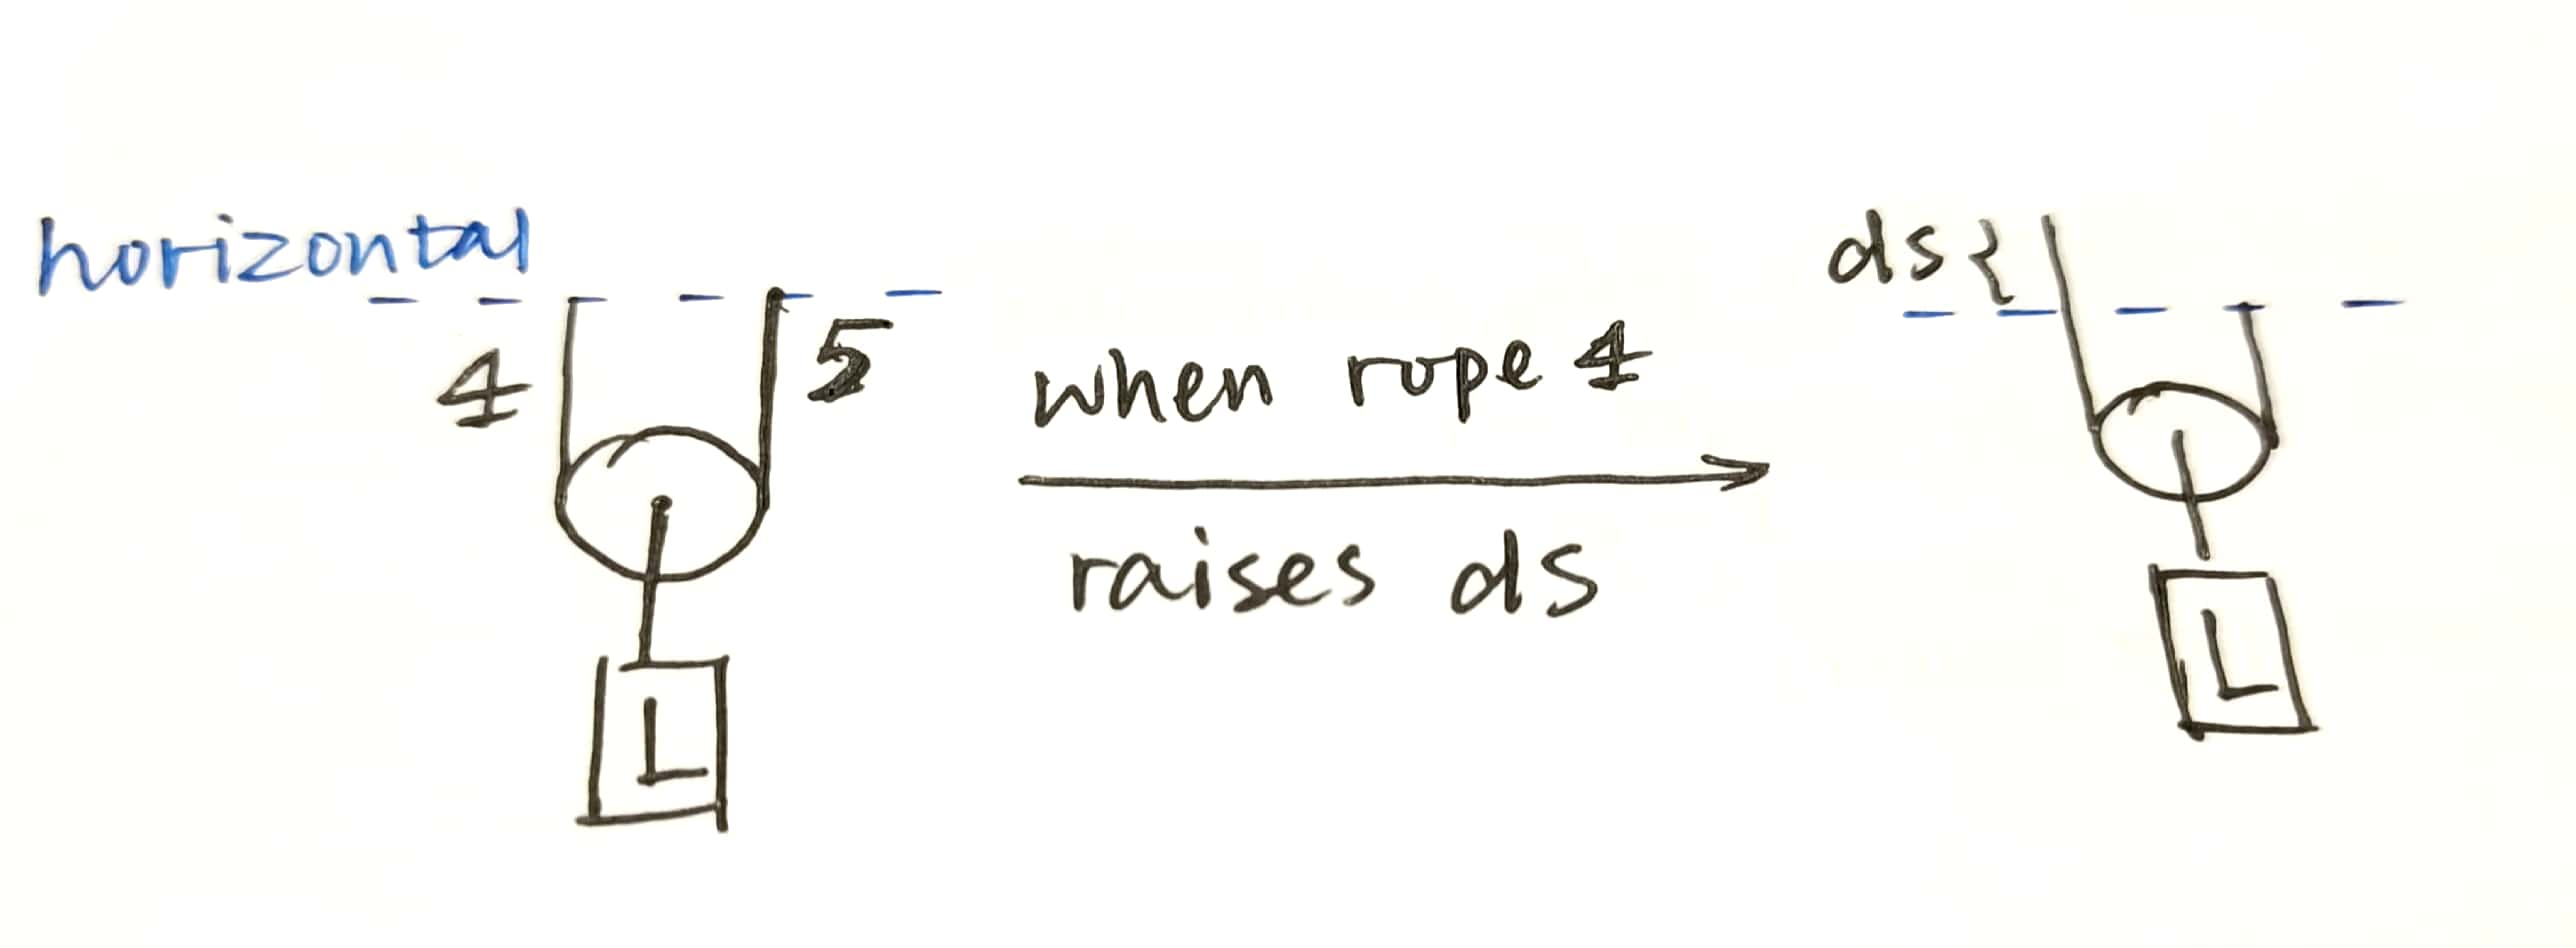
\includegraphics[height = 4cm]{2.jpg}
    \caption{Analysis of pulley attached to \textit{L}}
\end{figure}
\par It is also evident to see that cables below the horizontal line (blue line in Figure 2) raise $\frac{dS}{2}$ when cable 4 raises \textit{dS}.
\par Since all these movements occur in the same time period, the speed is directly proportional to the distance correspondingly. Therefore, we have
\begin{align*}
	v_B &= \frac{1}{3} v_M\\
	v_L &= \frac{1}{2} v_B\\
	\Rightarrow v_L = \frac{1}{6} v_M &= \frac{50}{3} \approx 16.7 \text{(mm/s)}
\end{align*}
\par Since \textit{L} moves upwards while the cable with $v_M = 100$ mm/s moves downwards, $\bar{v}_L = -16.7$ mm/s.

\paragraph{\large \textbf{Problem 2}}~{\textbf{Solution}}
\vspace{2mm}
\par We first select any instant t and let it be fixed. Then we can analyze both the dynamics and kinematics of this particle as follows.
\begin{figure}[H]
    \centering
    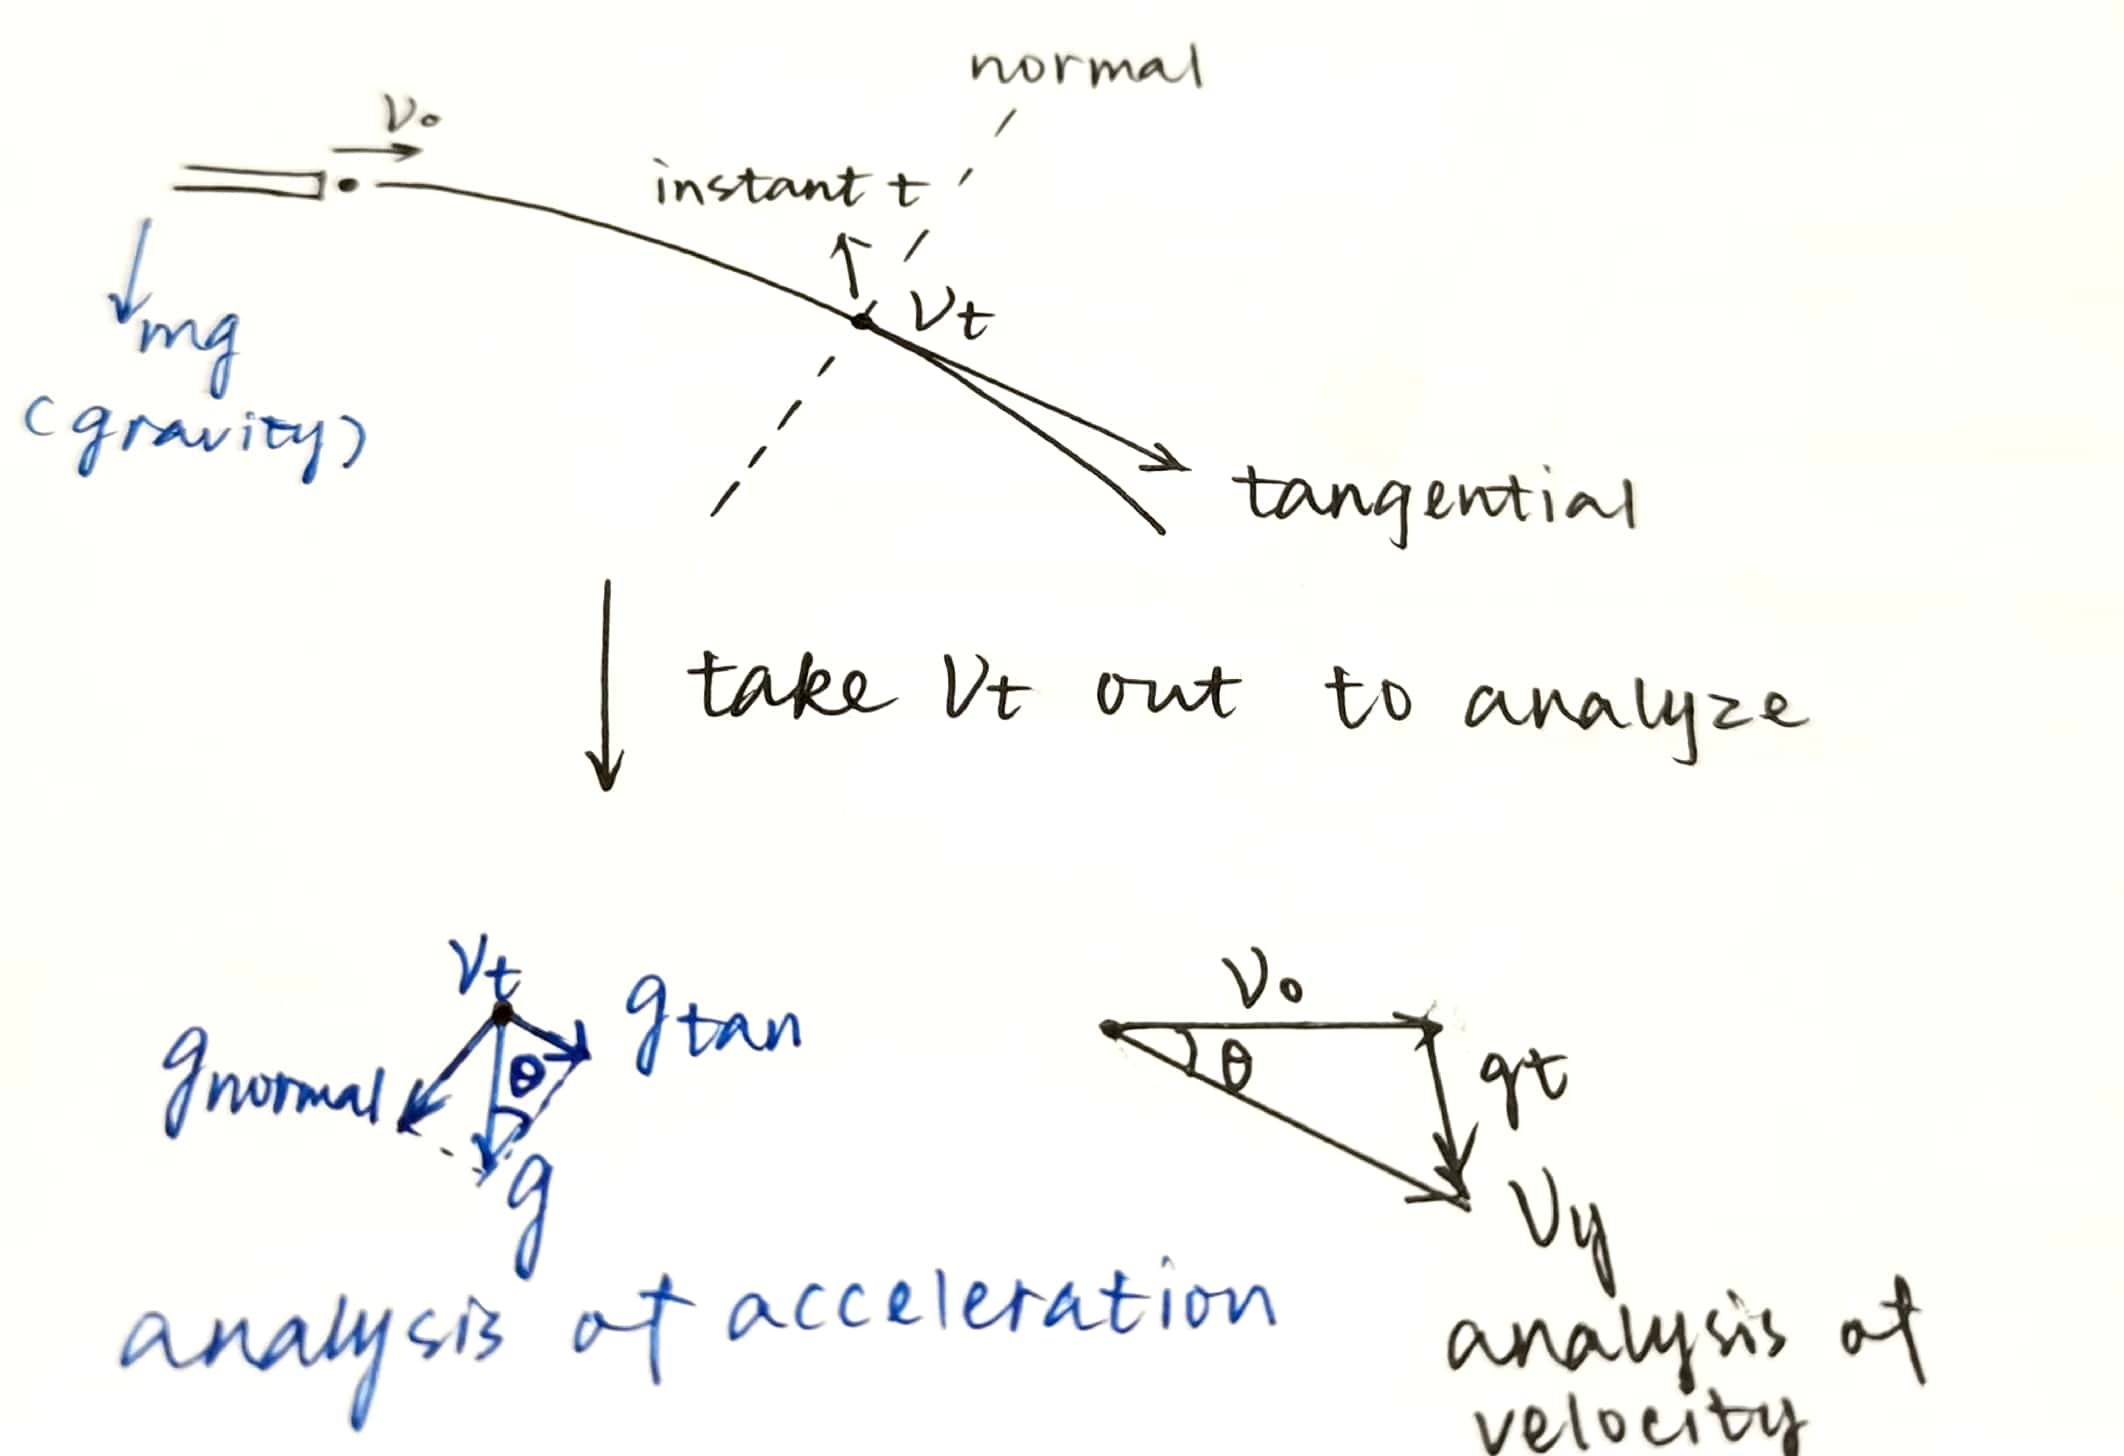
\includegraphics[height = 8cm]{3.jpg}
    \caption{Force analysis and kinematics analysis of the particle}
\end{figure}
\par To be more specific, we can conclude equations as follows
\begin{align*}
	\left\{ \begin{array}{c}
	\tan\theta = \frac{gt}{v_0}\\
	a_t = g\sin\theta\\
	a_n = g\cos\theta\\
	\end{array}	 \right.
\end{align*}
\par Solve this system we get
\begin{align*}
	\left\{ \begin{array}{c}
	a_t = \frac{g^2t}{\sqrt{g^2t^2+v_0^2}}\hat{a}_t\\
	a_n = \frac{gv_0}{\sqrt{g^2t^2+v_0^2}}\hat{a}_n
	\end{array} \right.
\end{align*}
\par Based on geometric triangles, we also know
\begin{align*}
	\bar{v}_y &= gt = a_t + a_n\\
\end{align*}

\paragraph{\large \textbf{Problem 3}}~{\textbf{Solution}}
\vspace{2mm}\\
\noindent (a) $\bar{v} = \bar{v}_1 + \bar{v}_2 = v_1\hat{n}_y + v_0\sin(\frac{\pi y}{L})\hat{n}_x$
\par $|\bar{v}| = \sqrt{v_1^2 + (v_0\sin\frac{\pi y}{L})^2}$\\
\noindent (b) When the canoe started from the southern bank, $y(t) = v_1t$, and when the canoe started from the northern bank, $y(t) = L-v_1t$. Then we apply integral
\begin{align*}
	x(t) = \int v_0\sin\frac{\pi y}{L} = v_0\int \sin\frac{\pi v_1 t}{L} = -\frac{v_0L}{\pi v_1}\cos\frac{\pi v_1t}{L}
\end{align*}
\par Therefore, trajectory $\bar{r}$ = (-$\frac{v_0L}{\pi v_1}\cos\frac{\pi v_1t}{L}$)$\hat{n}_x$ + $v_1t \hat{n}_y$ or $\bar{r}$ = (-$\frac{v_0L}{\pi v_1}\cos\frac{\pi v_1t}{L}$)$\hat{n}_x$ + $(L-v_1t) \hat{n}_y$\\
\noindent (c)
\begin{align*}
	x(t) = \int_0^t v_0\sin\frac{\pi y}{L} = v_0\int_0^t \sin\frac{\pi v_1 t}{L} = -\frac{L}{\pi v_1}\cos\frac{\pi v_1t}{L}|_0^{L/v_1} = \frac{2v_0}{\pi v_1}L
\end{align*}

\paragraph{\large \textbf{Problem 4}}~{\textbf{Solution}}
\vspace{2mm}
\par The units of \textit{b} and \textit{c} are $m$\\
\noindent (a) Since $x = r\cos\varphi$ and $y = r\sin\varphi$, we have
\begin{align*}
	\left\{ \begin{array}{c}
	r\cos\varphi = bt^2\\
	r\sin\varphi = -ct^2
	\end{array}	\right.
\end{align*}
\par Therefore, we get the parametric equations of the trajectory
\begin{align*}
	\left\{ \begin{array}{c}
	r = \sqrt{b^2+c^2} t^2\\
	\varphi = \arctan(-\frac{c}{b})
	\end{array}	\right.
\end{align*}

\noindent (b) Since $x(t) = bt^2$ and $y(t) = -ct^2$, $\frac{x}{y}$ = -$\frac{b}{c}$ $\Rightarrow$ $cx+by = 0$
\par Therefore, the implicit form in polar coordinate system is $cr\cos\varphi + br\sin\varphi = 0$\\
\noindent (c) In the Cartesian coordinate system, $v(x) = \mathop{x(t)}\limits^{\cdot} = 2bt$, $v(y) = \mathop{y(t)}\limits^{\cdot} = -2ct$. 
\par Therefore, $\bar{v} = 2bt\hat{n}_x - 2ct\hat{n}_y$, $\bar{a} = \mathop{\bar{v}}\limits^\cdot = 2b\hat{n}_x - 2c\hat{n}_y$
\par In polar coordinate system, $\bar{r} = r\hat{n}_r$, $\bar{v} = \mathop{\bar{r}}\limits^{\cdot}$ = $\mathop{r}\limits^{\cdot}\hat{n}_r + r\mathop{\hat{n}_r}\limits^{\cdot}$ = $\mathop{r}\limits^{\cdot}\hat{n}_r$ + $r\mathop{\varphi}\limits^{\cdot}\hat{n}_\varphi = 2\sqrt{b^2+c^2}t\hat{n}_r$, $\bar{a} = (\mathop{r}\limits^{\cdot\cdot} - r(\mathop{\varphi}\limits^{\cdot})^2)\hat{n}_r + (r\mathop{\varphi}\limits^{\cdot\cdot}+2\mathop{r}\limits^{\cdot}\mathop{\varphi}\limits^{\cdot})\hat{n}_\varphi$ = 2$\sqrt{b^2+c^2}\hat{n}_r$

\paragraph{\large \textbf{Problem 5}}~{\textbf{Solution}}
\vspace{2mm}
\par The unit of \textit{c} is $\frac{1}{s}$ while the unit of $r_0$ is \textit{m}. \\
\noindent (a) $\frac{r}{r_0} = 1 - ct$ $\Rightarrow$ $ct = 1 - \frac{r}{r_0}$ 
\par $\Rightarrow$ $\varphi = \frac{1-r/r_0}{r/r_0} = \frac{r_0-r}{r}$
\par In order to show helix trajectory completely, I limited the range of $\varphi$ in three ranges. Since the figure will become concentric circles when $\varphi$ is really large, I only drew the figure in a limited range.
\begin{figure}[H]
    \centering
    \subfigure[$\varphi$ ranges from 0 to 4$\pi$]{
    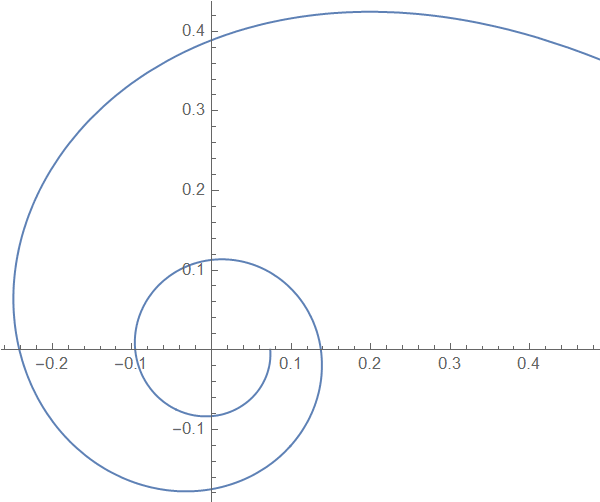
\includegraphics[height = 3cm]{1.png}
    }
    \subfigure[$\varphi$ ranges from 0 to 10$\pi$]{
    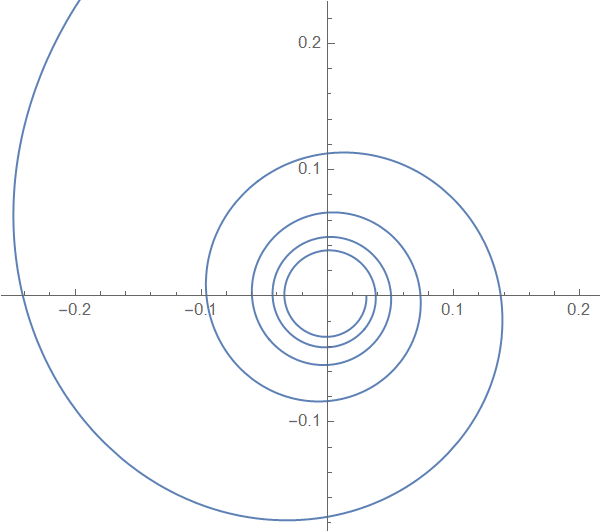
\includegraphics[height = 3cm]{2.png}
    }
    \subfigure[$\varphi$ ranges from 0 to 20$\pi$]{
    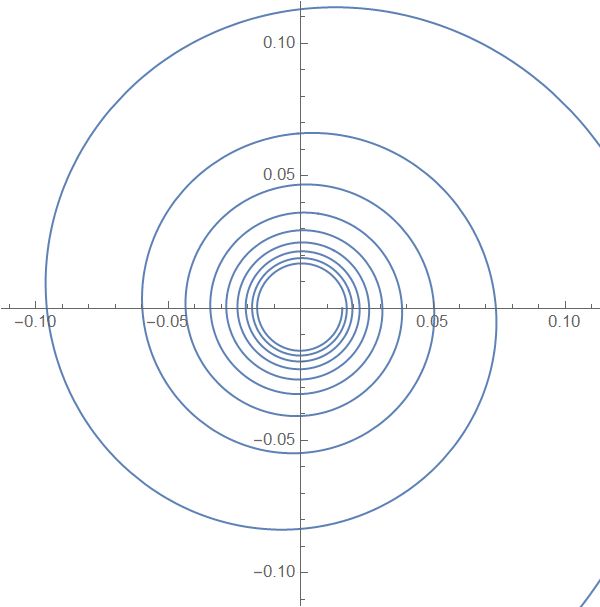
\includegraphics[height = 3cm]{3.png}
    }
    \caption{Trajectory of the particle}
\end{figure}
\noindent (b) $\bar{v} = \mathop{\bar{r}}\limits^{\cdot}$ = $\mathop{r}\limits^{\cdot}\hat{n}_r + r\mathop{\hat{n}_r}\limits^{\cdot}$ = $\mathop{r}\limits^{\cdot}\hat{n}_r$ + $r\mathop{\varphi}\limits^{\cdot}\hat{n}_\varphi$ = $-cr_0 \hat{n}_r + \frac{cr_0-c^2r_0t}{(1-ct)^2}\hat{n}_\varphi$ = $-cr_0 \hat{n}_r$ + $\frac{cr_0}{1-ct}\hat{n}_\varphi$\\
$v = \sqrt{(-cr_0)^2 + (cr_0/(1-ct))^2} = \lvert cr_0 \rvert \sqrt{1+(1/(1-ct)^2)}$\\
\noindent (c) $\bar{a} = (\mathop{r}\limits^{\cdot\cdot} - r(\mathop{\varphi}\limits^{\cdot})^2)\hat{n}_r + (r\mathop{\varphi}\limits^{\cdot\cdot}+2\mathop{r}\limits^{\cdot}\mathop{\varphi}\limits^{\cdot})\hat{n}_\varphi$ = $(-c^2r_0+c^3r_0t)/(1-ct)^4\hat{n}_r = -\frac{c^2r_0}{(1-ct)^3}\hat{n}_r$\\
\noindent (d) When \textit{c} $\textgreater$ 0, $\bar{a} \textgreater$0 as time goes by and $\bar{v}_r \textless$0. Therefore, the particle moves closer and closer, faster and faster to the origin and the acceleration increases.
\par When \textit{c} $\textless$ 0, $\bar{a} \textless$0 as time goes by and $\bar{v}_r \textgreater$0. Therefore, the particle moves farther and farther, slower and slower to the origin and the acceleration decreases.

\paragraph{\large \textbf{Problem 6}}~{\textbf{Solution}}
\vspace{2mm}\\
\noindent (a) The unit of $\frac{3}{\pi}$ is radian, the unit of $\pi$ is $s^{-1}$, the unit of 6 is \textit{cm}, the unit of 2 is $s^{-1}$.\\
\noindent (b) $\bar{v} = \mathop{\bar{r}}\limits^{\cdot}$ = $\mathop{r}\limits^{\cdot}\hat{n}_r + r\mathop{\hat{n}_r}\limits^{\cdot}$ = $\mathop{r}\limits^{\cdot}\hat{n}_r$ + $r\mathop{\varphi}\limits^{\cdot}\hat{n}_\varphi$ = $12e^{-2}\hat{n}_r + (18e^{-2}-18)\hat{n}_\varphi$
\par radial: $v_r$ = $\frac{12}{e^2} \hat{n}_r$\quad \quad transverse: $v_\varphi$ = $\frac{18}{e^2}-18 \hat{n}_\varphi$\\
\noindent (c) $\bar{a} = (\mathop{r}\limits^{\cdot\cdot} - r(\mathop{\varphi}\limits^{\cdot})^2)\hat{n}_r + (r\mathop{\varphi}\limits^{\cdot\cdot}+2\mathop{r}\limits^{\cdot}\mathop{\varphi}\limits^{\cdot})\hat{n}_\varphi$ = (30$e^{-2}-54$)$\hat{n}_r$ - 72$e^{-2}\hat{n}_\varphi$
\par ratial: $a_r$ = (30$e^{-2}-54$)$\hat{n}_r$\quad \quad tranverse: $a_\varphi$ = - 72$e^{-2}\hat{n}_\varphi$\\
\noindent (d) For the rod system, the collor moves along the rod so there is no $\varphi$ change. Therefore, $a$ = $a_{\text{ratial}}$ = (30$e^{-2}-54$)$\hat{n}_r$
\end{document}